% !TEX TS-program = pdflatex
% !TEX encoding = UTF-8 Unicode

% This is a simple template for a LaTeX document using the "article" class.
% See "book", "report", "letter" for other types of document.

\documentclass[11pt]{article} % use larger type; default would be 10pt

\usepackage[utf8]{inputenc} % set input encoding (not needed with XeLaTeX)

%%% Examples of Article customizations
% These packages are optional, depending whether you want the features they provide.
% See the LaTeX Companion or other references for full information.

%%% PAGE DIMENSIONS
\usepackage{geometry} % to change the page dimensions
\geometry{a4paper} % or letterpaper (US) or a5paper or....
% \geometry{margin=2in} % for example, change the margins to 2 inches all round
% \geometry{landscape} % set up the page for landscape
%   read geometry.pdf for detailed page layout information

\usepackage{graphicx} % support the \includegraphics command and options
\usepackage{caption}
\usepackage{subcaption}

% \usepackage[parfill]{parskip} % Activate to begin paragraphs with an empty line rather than an indent

%%% PACKAGES
\usepackage{booktabs} % for much better looking tables
\usepackage{array} % for better arrays (eg matrices) in maths
\usepackage{paralist} % very flexible & customisable lists (eg. enumerate/itemize, etc.)
\usepackage{verbatim} % adds environment for commenting out blocks of text & for better verbatim
\usepackage{cite}
% These packages are all incorporated in the memoir class to one degree or another...

%%% HEADERS & FOOTERS
\usepackage{fancyhdr} % This should be set AFTER setting up the page geometry
\pagestyle{fancy} % options: empty , plain , fancy
\renewcommand{\headrulewidth}{0pt} % customise the layout...
\lhead{}\chead{}\rhead{}
\lfoot{}\cfoot{\thepage}\rfoot{}

%%% SECTION TITLE APPEARANCE
\usepackage{sectsty}
\allsectionsfont{\sffamily\mdseries\upshape} % (See the fntguide.pdf for font help)
% (This matches ConTeXt defaults)

\usepackage{authblk} %Allow more complex author information

%%% ToC (table of contents) APPEARANCE
\usepackage[nottoc,notlof,notlot]{tocbibind} % Put the bibliography in the ToC
\usepackage[titles,subfigure]{tocloft} % Alter the style of the Table of Contents
\usepackage{subfig} % make it possible to include more than one captioned figure/table in a single float
\usepackage{amsmath}
\renewcommand{\cftsecfont}{\rmfamily\mdseries\upshape}
\renewcommand{\cftsecpagefont}{\rmfamily\mdseries\upshape} % No bold!

%%% END Article customizations

%%% The "real" document content comes below...

\title{A Game Theoretical Exploration of Open Science}
\author[1]{Robert Olendorf}
\author[2]{Steve Koch}
\affil[1]{University Libraries, University of New Mexico}
\affil[2]{Department of Physics and Astronomy, University of New Mexico}
%\date{} % Activate to display a given date or no date (if empty),
         % otherwise the current date is printed 

\begin{document}
\maketitle

%\section{}

The value of sharing data and other research products is increasingly recognized. Many funding agencies, such as NSF and NIH now require that data created through their grants be made available to others in a reasonable amount of time. Additionally, many journals now require or encourage that the data used as a basis for a manuscript be made available. Universities, including University of New Mexico, are working to create data repositories to help researchers make the products of their research available. 

While acknowledging the public good of making their data more avaialble, many if not most individual researchers are still reluctant to make their data available. There are several reasons for this attitude. First and foremost is researchers fear that others will publish from their data before them. Additionally, researchers worry that their data will be used without proper attribution and that their data will be misunderstood or used inappropriately. Essentially, researchers believe that while making their data more open may benefit society, there are few personal benefits and considerable personal risks to doing so. This dichotomy between the wish to make research more open for the public good, and to keep data closed for personal interest creates a tension between funding agencies, policy makers and others hoping to make research more open, and individual researchers who create the content.

In this manuscript we will use game theoretical arguments, specifically work based on the well researched Prisoners' Dilemma to explore how we can create an atmosphere where researchers feel they receive direct benefits to making their data more open. We will show that it is possible that even in the current environment openness in research direclty benefits researchers. We will also explore ways to further increase direct benefits to researchers. Finally, we will provide examples from our own experiences in open research, as well as experimental examples from the literature that show how openness can be encouraged.
\section{Theory}
\subsection{The Prisoners' Dilemma and Open Science}
\begin{figure}[ht]
	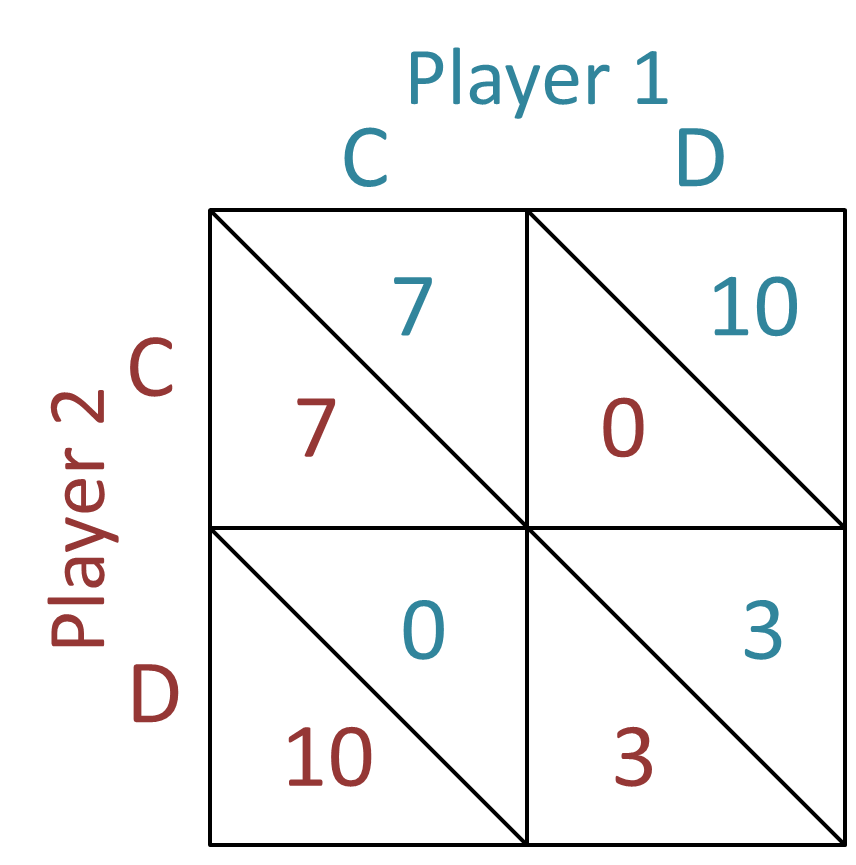
\includegraphics[width=0.5\textwidth]{files/figures/pdmatrix.png}
	\caption{A sample example matrix for the Prisoners' Dilemma. The players can either Cooperate(C) or Defect(D).  Numbers above the diagonal represent payoffs to Player 1, numbers below the diagonal represent payoffs to Player 2.}
	\label{pdmatrix}
\end{figure}
We will use the Prisoners' Dilemma to explore open science. The Prisoners' Dilemma is a game theoretical construct developed in the RAND corporation by Merrill Flood and Melving Dresher in 1950 \cite{ABAGFBEC19920101, unm.b196052419570101} to study situations where there is both a strong incentive to cooperate, but also a strong temptation to defect. Figure~\ref{pdmatrix} shows a specific example of the Prisoners' Dilemma (PD). In the PD each player can do one of two actions, Cooperate, or Defect (cheat). Mutual cooperation yields a relatively high reward. However, if a player can defect while the other player cooperates, they get an even higher reward (the big payoff) the other player gets the lowest possible payoff (the suckers payoff). There are a few constraints on the payoff matrix. The big payoff to a Defector against a Cooperator needs to be higher than mutual cooperation. If mutual cooperation is higher, then cooperating is always favored. Second, mutual cooperation must be higher than the average of the big payoff and the sucker's payoff. In the example shown in Figure~\ref{pdmatrix}, the payoff for mutual cooperation is seven, while the average of the big payoff and the sucker's payoff is 5 ((10+0)/2). This prevents an alternating strategy from being favored in the Iterated Prisoners' Dilemma discussed below.

If the game is to be played only once, then the only rational move is to defect. If Player 1 knows that Player 2 will cooperate, then she maximizes her reward by defecting and yielding 10. On the other hand, if Player 1 knows that Player 2 will defect, then she should still defect because then she will get at least 3 rather than 0. Player 2 follows the same logic and the equilibrium is for both players to defect. This is known as a Nash Equilibrium, defined as a situation when neither player benefits by changing strategies \cite{unm.b196052419570101}.

The Prisoners' Dilemma serves as a useful paradigm for exploring open research for a number of reasons. First, is often the model used to explore situations where individuals must trade personal gain for a public good. More importantly, if as we will argue, that open research presents both personal rewards as well as risks, this model captures this dynamic.

\subsection{Tit-For-Tat}
If the game is to played for some unknown number of times (Iterated Prisoners' Dilemma or IPD), then the situation becomes much more complicated because the players are now able to base their decisions both on past behavior and expectations of future behavior. It is important that the number of interactions is not known to the players, otherwise the last interaction is played just like a single play Prisoners' Dilemma and both players defect. Since both players know that the last move is to defect, they use similar logic on the second to last interaction, continuing until the first interaction where both players defect.

 In 1981  Axelrod and Hamilton \cite{axelrodhamilton1981} conducted a tournament where strategies for playing the IPD were pitted agains one another. Surprisingly, the simplest submission won, Tit-For-Tat (TFT). The TFT strategy cooperates on the first move than simply repeats the other player's last move thereafter. Subsequent analysis and tournaments suggest that TFT is successful because of three traits. First it is nice in that the first move is cooperative by default. Second, it is retaliatory, in that defection is the next move after the other player defects. Finally, it is forgiving because cooperation follows if the other player then cooperates on future moves. Subsequent work has shown that other successful strategies also share these traits
\cite{axelroddion1988, ABAGFBEC19920101, unm.b685148920000101}.
\subsection{Population Dynamics}
In most cases players are not just playing agains one player, but exist in a population of players. We must therefore consider the dynamics of strategies in the IPD played against a population of strategies. To do this we must redefine our equlibrium from a situation where neither player benefits by changing strategies to the situation where a population of players cannot be invaded by any alternative strategy that is initially rare. This is known as an Evolutionarily Stable Strategy (ESS) first developed by J. Maynard Smith \cite{smithprice1973}. An ESS is actually a Nash equilbirium extended for the case of a population rather than two individuals. 

\begin{figure}[ht]
	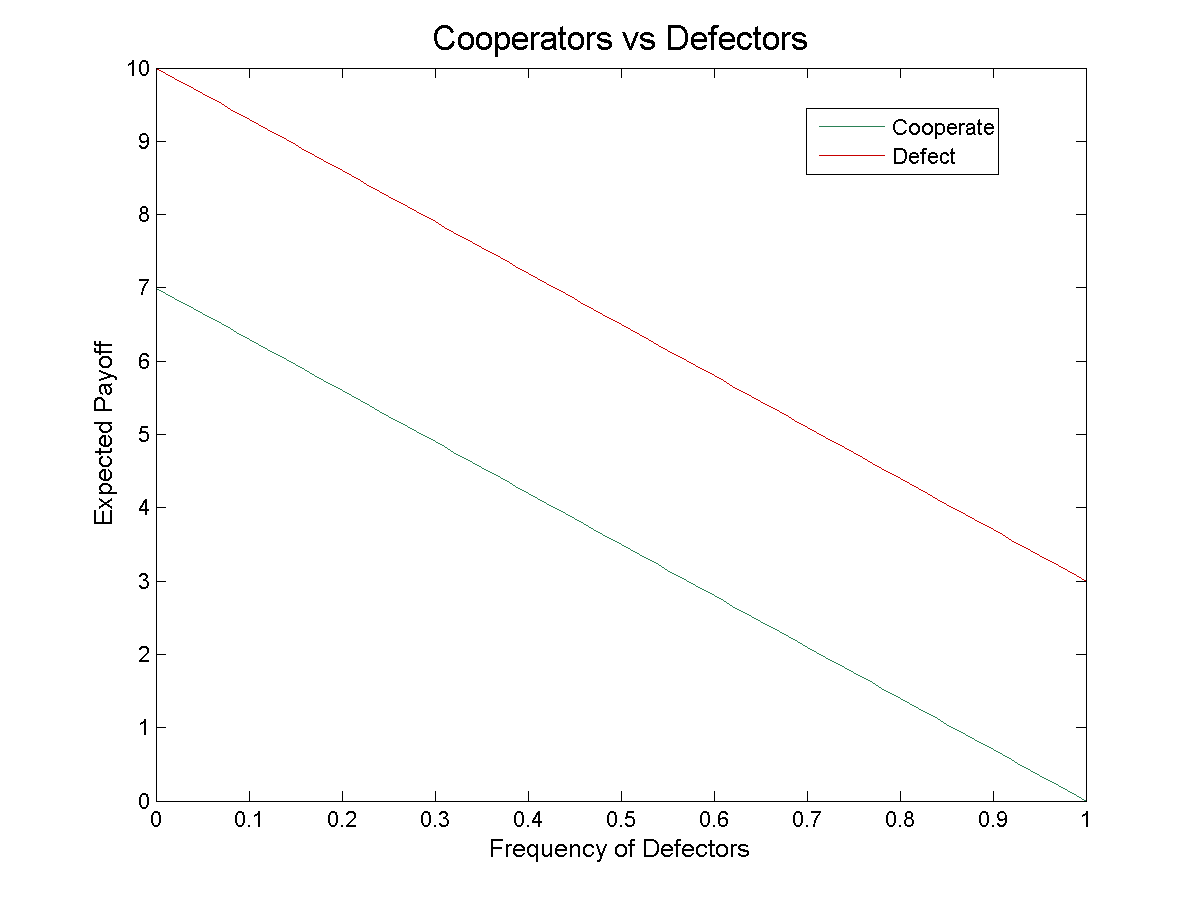
\includegraphics[width=0.7\textwidth]{files/figures/DvsC.png}
	\caption{The payoffs to Cooperate and Defect strategies as a function of the frequency of Defectors in the population.}
	\label{cvsd}
\end{figure}

We can determine the expected payoff for each interaction to each strategy with the following formulas. We use the payoff per interaction to allow us to compare between long and short expected numbers of interactions. For each strategy, we simply sum the expected payoff per interactoin to that strategy multiplied by the frequency of each strategy. We define $\mu$ as the expected number of plays or interactions in a game,  $\omega_{x}$ is the expected payoff to strategy x, $ F_{x}$ is the frequency of strategy x in the population and $P_{XY}$ is the payoff to Player Y when the other Player plays X. In the simplest case of a population of pure Cooperators and Defectors we get
\begin{subequations}
	\begin{equation}
	\omega_{D(d\_vs\_c)} = \frac{\mu * (1-F_{D})(P_{CD}) + F_{D } * P_{DD}}{\mu}
	\end{equation}
\mbox{ $\mu$ cancels out so the payoff is independent of the number of times the players expect to interact.}
	\begin{equation}
	\omega_{D(d\_vs\_c)} = (1-F_{D})(P_{CD}) + F_{D } * P_{DD}
	\label{d_in_dvsc}
	\end{equation}
\end{subequations}
and likewise, the expected payoff to Cooperating is
\begin{equation}
	\omega_{C(d\_vs\_c)} = (1-F_{D})(P_{CC}) + F_{D } * P_{DC}
	\label{c_in_dvsc}
\end{equation}

In the case of a Cooperators and Defectors we can see in Figure~\ref{cvsd} that while the expected payoff to both strategies decreases as the number of defectors increases. Also, both strategies achieve a higher payoff in an environment with more Cooperators, but because Defectors always achieve a higher payoff the population is only stable with pure defection. This is essentially the same result as we saw with only two players.

\begin{figure}
	\begin{subfigure}[b]{0.55\textwidth}
		\centering
		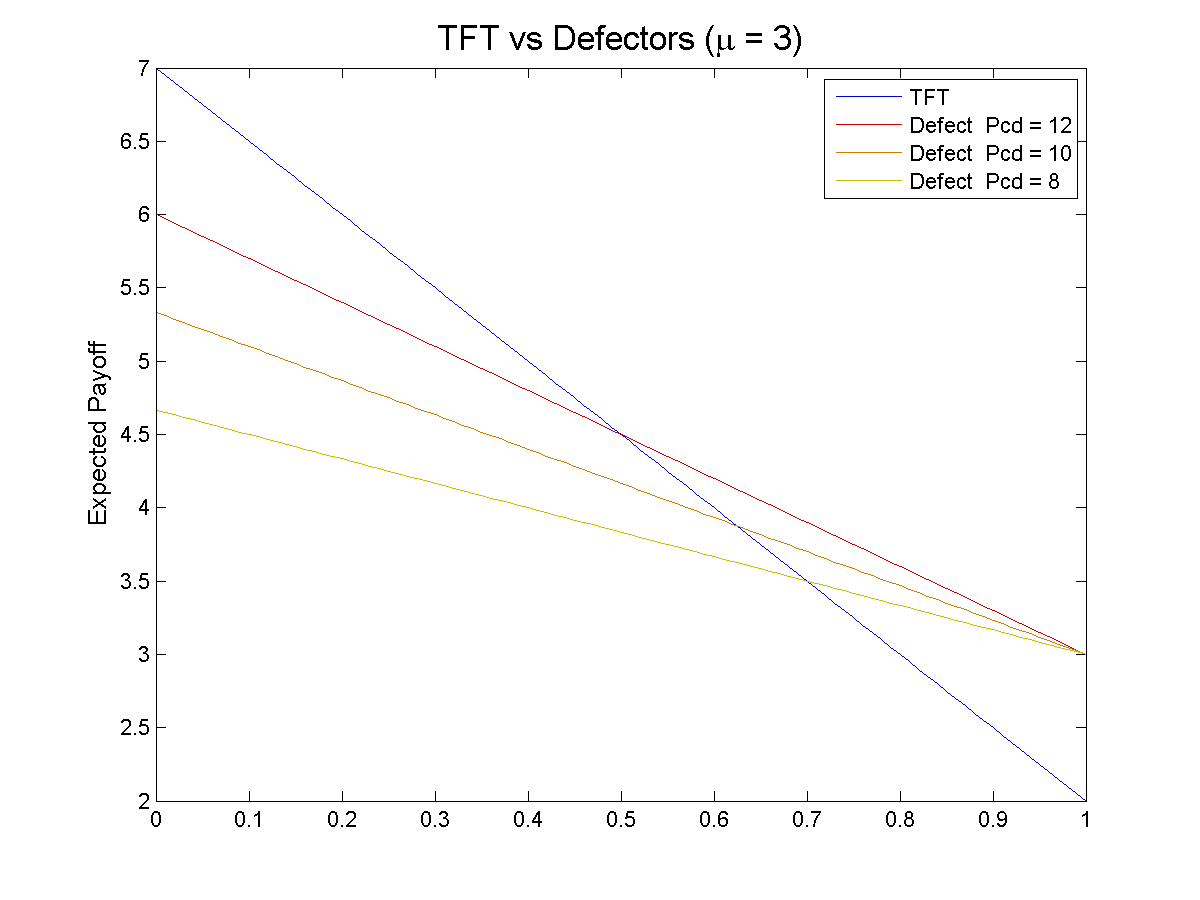
\includegraphics[width=\textwidth]{files/figures/DvsTFT_mu3}
		\caption{Expected number of interactions = 3.}
	\end{subfigure}
	\begin{subfigure}[b]{0.55\textwidth}
		\centering
		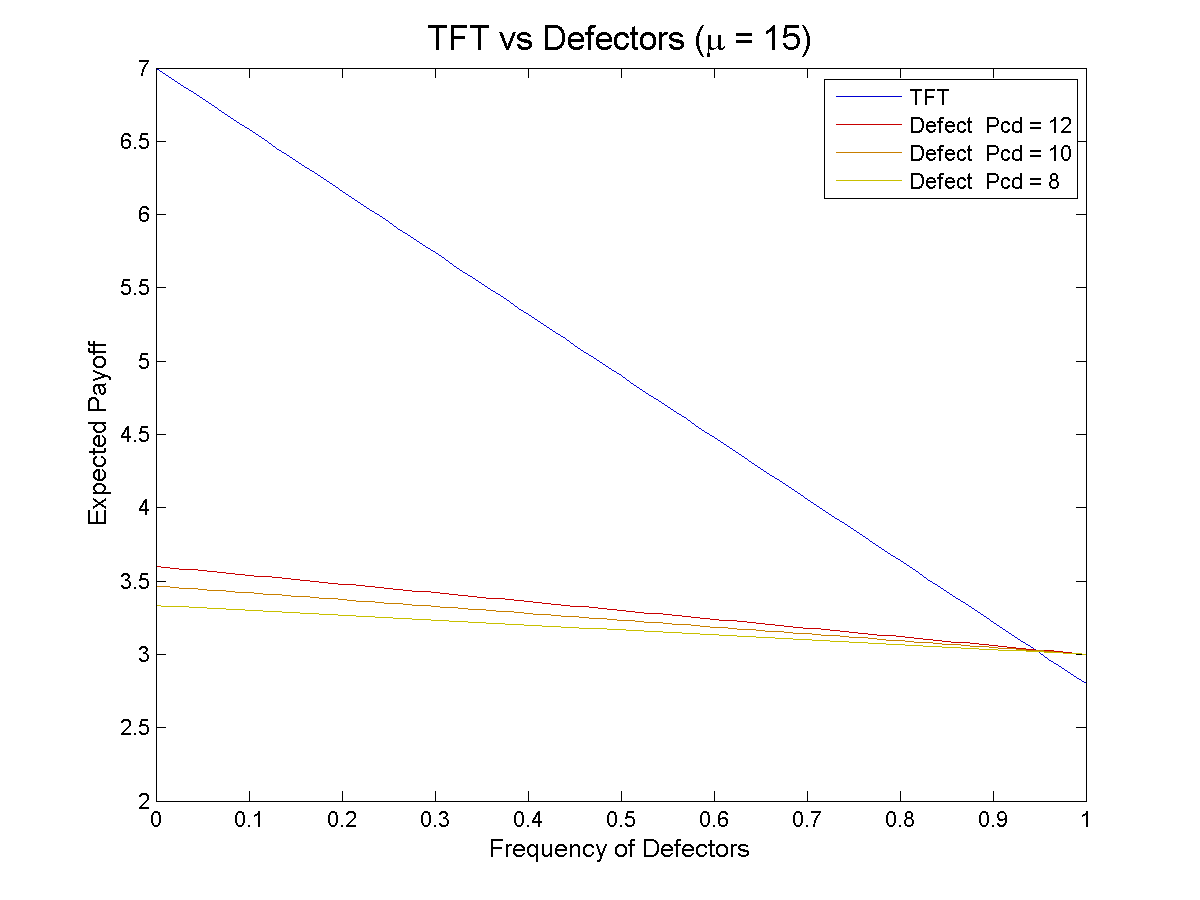
\includegraphics[width=\textwidth]{files/figures/DvsTFT_mu15}
		\caption{Expected number of interactions = 15.}
	\end{subfigure}
	\caption{The expected payoff per interaction as a function of the frequency of defectors. The intersection
		    between the blue (TFT) line and the red-orange lines represent critical points. If the frequency
		    of defectors is higher than the critical value, then defectors will be favored, while if the
		   frequency of defectors is less than the critical point TFT will be favored. Moving the critical point
		  to the right favors TFT, meaning that lowering the payoff for defecting against a cooperation, and
	            increasng interactions favor TFT.}
	\label{tftvsd}
\end{figure}


We approach determining the payoffs in a population of Defectors and TFT strategists in a similar way.
\begin{equation}
	\omega_{D(d\_vs\_tft)} = \frac{(1 - F_{D})(P_{CD} + (P_{DD} * (\mu - 1)))}{\mu} + F_D * P_{DD}
	\label{d_in_dvstft}
\end{equation}
and  the payoff to TFT is
\begin{equation}
	\omega_{TFT} = (1-F_{D}) * P_{CC} + \frac{F_{D} * (P_{DC} + (\mu - 1) * P_{DD})}{\mu}
	\label{tft_in_dvstft}
\end{equation}

There are a number of things to notice. First, as shown in Figure~\ref{tftvsd}, Defectors are not always favored. When the TFT line is above the Defectors line, TFT is favored and eventually come to dominate the population at equilibrium. The point where the lines cross is a threshold point. If the frequency of Defectors is less than this point, TFT will be favored and come to dominate, while if the frequency of Defectors is higher than this point, Defectors are favored. This interaction derives from the fact that while Defectors enjoy a long string of high payoffs against Cooperators, they only enjoy this high payoff once against TFT strategists. Similarly, TFT strategists only suffer the suckers payoff once against a Defector, while a Cooperator endures a potentially long string of suckers payoffs.  Also, we can see that increasing the temptation to cheat (i.e., increasing the ``big payoff''), makes defection more likely, while increasing the benefit to ``mutual coopeartion'' makes TFT more attractive. 

\begin{figure}[ht]
	\centering
	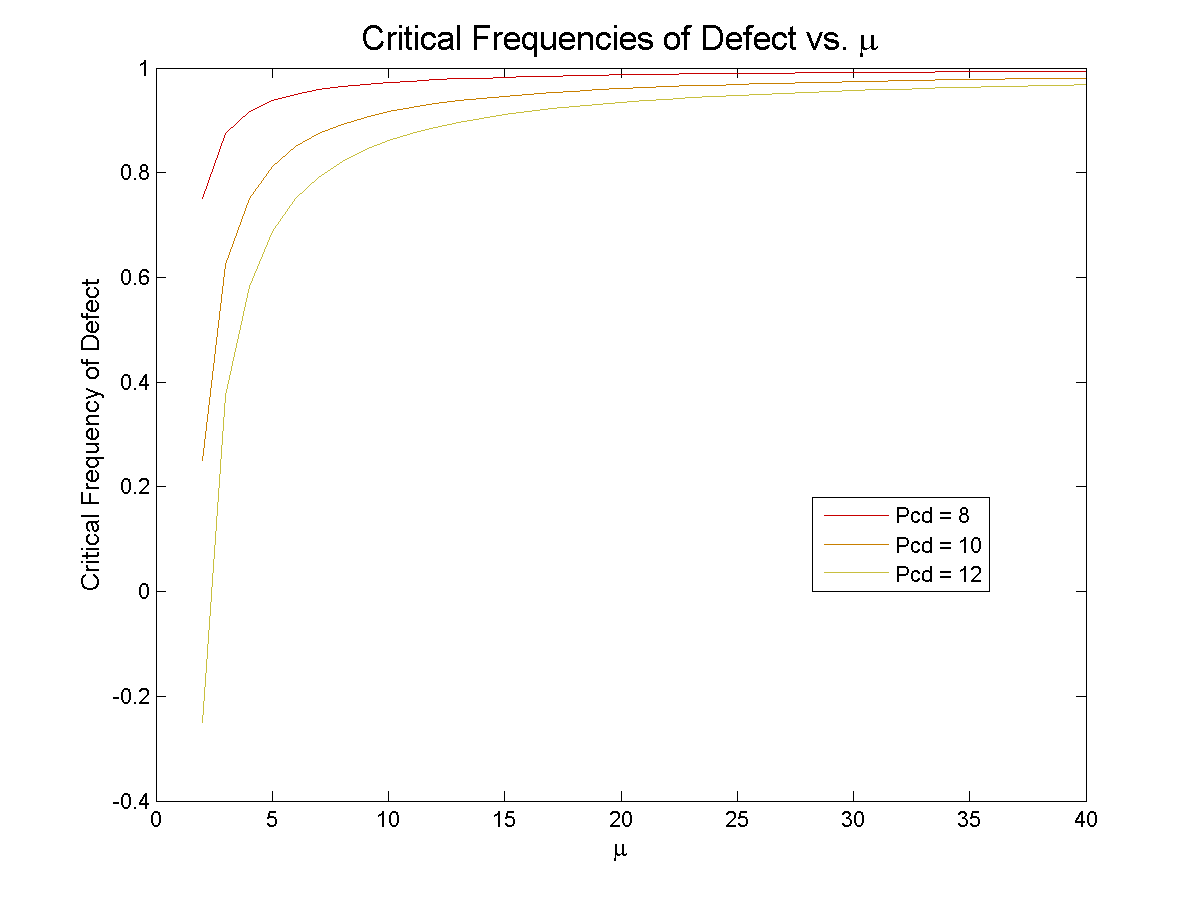
\includegraphics[width=0.85\textwidth]{files/figures/fdcrit.png}
	\caption{The affect of increasing expected interaction length in TFT versus D populations.}
	\label{muintft}
\end{figure}

Extending this affect is the influence the expected interaction length has on the threshold point.  Figure~\ref{muintft}, shows how with very short expected interaction lengths, the threshold for Defectors to dominate is very low, while increasing the expected interaction length rapidly increases this threshold. This results from the fact that Defectors only get one big payoff on their first interaction with a TFT. Thereafter, both TFT and Defectors defect realizing a relatively low payoff. At the same time, TFT only get the suckers payoff once, and thereafter get the low, but still higher, mutual defection payoff. The longer two players interact, the less important the initial payoff becomes to each player and the affect of the mutual defection payoff dominates the mean payoff.

Also, as shown in Figure~\ref{tftvsd} the temptation to defect (the payoff to a player when she defects while the other player cooperates) influences this threshold. The higher the temptation to defect, the lower the threshold value is meaning that Defectors are favored at a lower frequency. Also, while the expected number of interactions with another player was not an issue when Defectors and Cooperators were competing ($\mu$ cancels out in equations~\ref{d_in_dvsc} and \ref{c_in_dvsc}), the expected number of interactions is a factor when TFT and Defectors compete. 

\subsection{Caveats}
There are two fairly obvious implicit simplifications to this model that must be addressed. First, the payoffs in the Prisoners' Dilemma as described are static, while in reality, the payoffs are probably often continuous and vary depending on the players' behaviors. The Continuous Prisoners' Dilemma has been a recent topic of theoretical research, and to summarize the overall conclusions, the basic conclusions remain the same. However, stable cooperative equilibria are more difficult to achieve without adding additional factors such as cooperators favoring other cooperators to interact with \begin{em}cite some of the recent theoretical work here\end{em}. Additionally, there are a number of empiricle examples of cooperative and tit-for-tat like behavior in the natural world where the underlying model is mostly continuous \begin{em}cite olendorf, milinksi etc here\end{em}.


\section{Discussion}
We will now explore how the Prisoners' Dilemma can inform how researchers, institutions, funding agencies, journals and other interested parties currently practice research and how they can modify their behaviors to favor a more open environment in research. We will first describe how the payoff structures and strategies described above apply to open research. We will discuss how current research practices affect openness and how we can increase the level of openness in research. We will focus primarily on the payoffs to individual researchers as they are the creators of the data and other products of researcher.

While the motivations and rewards of research probably vary somewhat from researcher to researcher, here we will assume that the primary component of the payoff is tenure and promotion. Factors that enhance the chances of gaining tenure and promotion increase the payoff, while factors the reduce the chances of tenure and promtion will reduce the payoff. Making this assumption probably captures a large part of what a vast majority of researchers care about when making decisions and it is probably also the biggest unifying facet of any researcher's career. Although other factors do go into the tenure and promotion process, such as teaching and service, we assume that they are not affected by open research.  At most research institutions, the publications and grants are the most important. We recognize that quantifying the costs and benefits is nearly impossible, however, we do believe this to be an excellent framework both for examining the current research environment, and also for exploring ways to change practices to facilitate greater openness.

Each payoff can be decomposed into costs and benefits. Mutual defection ($P_{DD}$) is what we  consider the traditional closed research model. The benefits are the publications and grants they receive either as an individual or with their collaborators, with very little direct costs. This payoff serves as our baseline payoff. 

A open research model is represented by mutual cooperation. As described above, to fit the Prisoners' Dilemma, the benefits to mutual cooperation must be higher than mutual defection. Under the current research environment, we are unsure if this is true, although in our personal experiences we have experienced benefits not realized in the tradional research model. One author (Steve Koch), runs an open science lab. Typically, data is created and made publicly available within a few days. Additionally, he and his students maintain active blogs as well as other social media feeds. In one case, data that was made publicly available , and adverstised on YouTube \cite{koch_kochlab, maloney_koch} was discovered by another researcher in a different field. This interaction led to a publication \cite{deutsch_mechanics_2011} which Koch and Maloney were invited to coauthor (an offer which they graciously refused in favor of an acknowledgement and a nod to open science)\cite{koch_steve_2011}. This experience demonstrates that the additional direct benefits to open science may include a higher publication rate, both directly and through the identification of new collaborators. Additional collaborators can also help in gaining more grants. Other benefits to open research are highighted by this manuscript. We made the decision to make this manuscript and all the supporting information open through GitHub\cite{olendorf_gtos_github} and to publicize it through social networks. Almost immediately after our first bit of work, we received a number of helpful suggestions and anticipate more in the future. We believe this process will result in a higher quality manuscript and a faster review process which ultimately will increase our publication rate.  Journals and funding agencies should also take a larger and more positive role in promoting open research. For instance, funding agencies should favor grants to researchers with a record of good open research.

Perhaps the most obvious cost to the open science model is the possibility that a researchers work will be misued or stolen and this is typically one of the first worries voiced by many researchers. While this is a risk, we feel this risk is overestimated in the minds of most. First, this risk also exists with closed research, although probably at a lower level. More importantly, researchers are actually protecting themselves by opening up their work and advertising their work. Essentially they have claimed some degree of primacy and also protected themselves by copyright and creating a number of external witnesses to the existence and ownership of the work. A related cost associated with this concept however, is the cost of being vigilant and protecting ones work and also. Other additional costs are time spent promoting ones work as well as additional time spent organizing and curating data and other products so that it is understandable to others. This cost of vigilance, especially of other peoples work, may be one of the more important factors in increasing openness in research. Recent work has shown that associating positively with other cooperators promotes cooperation. Additionally, there is some evidence that red-winged blackbirds attend to what their neighbors are doing and reacting negatively to defections their neighbors make with other neighbors \cite{olendorf_2004b}.

Despite the potential benefits to mutual cooperation in open research already discussed, most researchers still perceive that the overall costs to opening their research outweighs the benefits. This is quite possibly true. Funding agencies and journals cite the common good associated with open science as justification for requiring data and other products be made available and the example with the Koch's data certainly supports this stance. However, these institutions are relying on increasing the costs of not cooperating (withholding of further funding, or refusal to publish manuscripts) to promote openness. These policies probably make sense from the point of view from the agencies, because their reward is different than that of the individual researchers who created the content. We believe it would be more advantageous to direclty reward researchers for openness. For instance, promotion and tenure currently relies mostly on publicaitons and grants and puts little if any weight on other products of research such as data. This is partly cultural, however there are some practical reasons for this. Tenure and promotion committees can rely on the fact that manuscripts and grants are reviewed favorably before they are published or funded. Additionally, they can obtain metrics such as impact factor and number of citations for a published manuscript. To accomplish this, services such as data citation and data use metrics are needed.

We have made a case that mutual cooperation in the form of open science is potentially, if not already, advantageous. However, there are two strategies that mutually cooperate at equilibrium, Cooperate and TFT. There are some surprising differences between the two. We know from the previous discussion of the Prisoners' Dilemma that Cooperate always loses to Defect, so we would expect TFT to be the dominant strategy. In fact, Cooperate almost always facilates the domination of Defect in a population.  First lets suppose we have a population of TFT strategists. If some Cooperate strategists enter the population, they will be indistinguishable to the TFT strategists because everyone is still cooperating. However, if some Defect strategists enter the population, they will benefit from the Cooperators and the benefit is greater the more cooperators exists, potentially destabilzing the TFT equilibrium \begin{em} add the math here to support this \end{em}. However, given the discussion of costs and benefits above, we can also suspect that Cooperators are actualy avoiding some of the costs of TFT such as vigilance. In this case, Cooperators might actually have a higher payoff than TFT strategists in a population with a low frequency of Defectors. Since their payoff is higher, they would increase in numbers and eventually come to dominate. At some point, the frequency of Cooperators would be high enough that the population is now vulnerable to invasion by Defectors. In a sense, we can think of the Cooperators in this scenario as another type of defector, avoiding the costs associated with TFT. In fact, the Payoff matrix really just becomes another Prisoner's Dilemma. Therefore, although it might seem to be a good idea to be a Cooperator to facilitate Open Science, in fact its better to be a TFT strategist and pay some of the costs (if any) associated with the strategy.

Another avenue to facilitating cooperation is to reduce the ``big payoff'' awarded to defectors when playing against a TFT or Cooperator. The solution has already been discussed above to some extent. Defectors must be punished and TFT strategists must be vigilant and willing to punish the defectors, especially those using data and other work dishonestly. Reducing the ``big payoff'' may not be practical or even fair for the Defectors who are really just honest researchers following the closed science model, although social pressure on closed researchers using open data might be of use.

\section{Conclusions}
Funding institutions and journals and a small number of researchers are increasingly taking a stance toward open research. However, most researchers still feel that being too open with their research can harm their careers, and that open research is a risk they are unwilling to take. We used the Prisoners' Dilemma as a framekwork to explore the dynamics of open versus closed research. We argue that there are many benefits to open research that many researchers may not recognize. Additionally, we discussed a number of changes that funding agencies, universities and researchers can make to the culture of research that will promote a culture of openness in research. Additionally, we provide two instances where openness has only positive effects from our own experiences. Most people agree that greater access to the products of publicly funded research is a common good. However, we argue that the current culture of requiring openness while at the same time not providing additional benefits to openness is detrimental to open research. Instead, changes should be made in how research is practiced and how researchers are rewarded for their work so that researchers with an open research program flourish.



\bibliographystyle{plain}

\bibliography{refs}
\end{document}
